\documentclass[a4paper,11pt]{article}
\usepackage[english]{babel}
\usepackage[utf8]{inputenc}
\usepackage{amsmath}
\usepackage{threeparttable}
\usepackage{amsthm}
\usepackage{amsfonts}
\usepackage{amssymb}
\usepackage{graphicx}
\usepackage[boxed]{algorithm}
\usepackage{algorithmic}
\usepackage[natbib=true,sorting=none]{biblatex}
%\usepackage{fancyhdr}
%\usepackage{natbib}
%\usepackage[natbib=true]{biblatex}
%\usepackage{epstopdf}
%\usepackage{float}
%\usepackage{url}
\usepackage[pdftex]{hyperref}
\usepackage{enumerate}
\usepackage{array,ragged2e}

\newcommand{\R}{\mathbb{R}}
\newcommand{\N}{\mathbb{N}}
\newcommand{\Z}{\mathbb{Z}}
\newcommand{\C}{\mathbb{C}}
\newcommand{\dx}{\, \mathrm{d}}
\newcommand{\de}{\partial}

\newcolumntype{C}[1]{>{\Centering}m{#1}}

\newtheorem{thm}{Theorem}[section]
\renewcommand{\qedsymbol}{$\lozenge$}

%\bibliographystyle{unsrt}

%\hoffset = 0cm
%\voffset = -2cm
%\textheight = 700pt
%\marginparwidth = 0pt
%\textwidth = 450pt
%\oddsidemargin = 0pt
%\evensidemargin = 0pt
%\topmargin = 0pt

\renewcommand{\algorithmicrequire}{\textbf{Input:}}
\renewcommand{\algorithmicensure}{\textbf{Output:}}

\setlength\parindent{0pt}
\setlength{\parskip}{5pt} %%distanza fra i paragrafi

\bibliography{fft2d}

\begin{document}

\title{Bulk Synchronous Parallel implementation of the 2-Dimensional Fast Fourier Transform}
\author{Davide Taviani\\
(d.taviani@students.uu.nl)}
\date{19 January 2012}

\maketitle

\begin{abstract}
This report focus on the parallelization of the 2-Dimensional Fast Fourier Transform using the Bulk Synchronous Parallel programming model. After a brief introduction on the Discrete Fourier Transform and Fast Fourier Transform, two different approaches to its implementation are discussed and their BSP cost analyzed. In addition, some numerical experiment help us evaluate our theoretical analysis and understand when a parallel approach is convenient and to what extent.
\end{abstract}

\tableofcontents

\pagebreak

\section{Introduction}
In the field of Digital Signal Processing, when dealing with periodic functions that represent signals or images, a very important role is played by Fourier Analysis, a branch of Mathematical Analysis that studies the decomposition of functions into their frequency components.

With such a decomposition, we are able to effectively remove desired frequencies (which, for instance, correspond to noise in a image) o enhance some others; its application really are countless and affect, on a daily basis, almost everyone.

To give a formal definition of our framework, following the scheme of \citep{parsc}, let $f:\R \to \C$ be a $T$-periodic function, i.e. such that $f(t+T) = f(t)\;\forall t \in \R$.

The \textbf{Fourier Series} associated with $f$ is

\begin{align}
\label{fserie} \tilde{f}(t) = \sum_{k=-\infty}^{+\infty} c_k e^{\frac{2\pi i k t}{T}}
\end{align}

where the Fourier coefficient $c_k$ are given by

\begin{align}
\label{coeff} c_k = \dfrac{1}{T} \int_0^T f(t) e^{\frac{2\pi i k t}{T}} \mathrm{d}t
\end{align}

and $i$ represents the complex number such that $i^2 = -1$.

We can see that in order to compute $c_k$, we must deal with an integral; in every real world application, however, dealing with the continuous is not possible, and we must necessarily discretize. For this reason, one of the most important concepts in Fourier Analysis is the so-called \textbf{Discrete Fourier Transform} (DFT), which is the discrete analogous of the Fourier Transform.

As previously mentioned, our goal is to manipulate signals in some way: to do so, however, we must first be able to extract the required information from the signal, and this is where the DFT comes at play. For a more comprehensive overview of the meaning and the application of the DFT see \citep[p.~151]{parsc}, and \citep{hunt}.

In practice, such operator transforms a discrete, complex vector $x \in \C^n$ (which for example represents a sampling of someone's voice) in the vector $y \in \C^n$ in the following way \citep[p.101]{parsc}:

\begin{align}
 \label{dft} y_k = \sum_{j=0}^{n-1} x_j  e^{\frac{2\pi ijk}{n}} \qquad 0 \leq k < n
\end{align}

Furthermore, often it is convenient to express the DFT algorithm using a matrix notation, introducing the concept of the Fourier matrix\citep{tesi,parsc}.

If we consider the $n$-th root of unity

$$\omega_n =  e^{\frac{2\pi i}{n}}$$

the formula \eqref{dft} can be restated in the following, more common, way:

\begin{align}
 \label{dft2} y_k = \sum_{j=0}^{n-1} x_j  \omega_n^{jk}
\end{align}

It is fairly easy to see that, even under the assumption that $\omega_n^m$ has been pre-computed for all required $m$ and stored on a table, the cost of the straightforward computation of the DFT is still $8n^2-2n$ flops \citep[p.~102]{parsc}, therefore less than desirable for most cases.

For example, using \eqref{dft2} to perform the decoding of 0.74 seconds of music from a CD Audio, thus with a vector length of $n=32768$, 43 minutes are needed on a 3.3 Mflop/s computer. Such performance is far from impressive, since ideally everything should be done in real-time to listen continuously to music.

To solve this inconvenience, an algorithm for the fast computation of the DFT has been devised (it was discovered in its most basic by Gauss in 1805, too early to benefit from it). The rediscovery by Cooley and Tukey \citep{cooleytukey} is the most widespread (it is from the 1965, already in the era of digital computing) and goes by the name of \textbf{Fast Fourier Transform} (FFT), which has the much reduced cost of $5n \log_2 n$ flops; with this algorithm, the previously mentioned decoding from an audio CD can be done in real time.

In a vast amount of real world applications, the core of the computations are essentially FFTs; for this reason in many cases further improvements in its computation speed are very welcome; this is the main reason for a parallel approach toward the computation of such FFT: doing so, we are in fact effectively able to solve bigger instances in less time.

In particular, our interest is directed toward the parallelization of the FFT using the Bulk Synchronous Parallel programming model proposed by Valiant \citep{bsp}; for this reason, we closely follow the scheme outlined by Rob H. Bisseling in \citep{parsc}, where an implementation of the FFT, together with a wide analysis of the costs, is provided.

In the next section we focus on the parallelization of the 2-Dimensional FFT, which can find its application in the vast field of Digital Image Restoration; in particular, we proceed to study two possible extension of the function \verb|bspfft| found in \verb|BSPedupack| \citep{bspedupack}.


\section{Parallel 2-Dimensional Fast Fourier Transform}
The 2-Dimensional Discrete Fourier Transform (2D DFT) of an $n_0 \times n1$ matrix $X$ is defined as the $n_0 \times n_1$ matrix $Y$ given by:

\begin{align}
 \label{2dft} Y(k_0,k_1) = \sum_{j_0=0}^{n_0-1} \sum_{j_1=0}^{n_1-1} X(j_0,j_1) \omega_{n_0}^{j_0 k_0} \omega_{n_1}^{j_1 k_1}
\end{align}

where, similarly as before, $\omega_n$ denotes the $n$-th root of unity.

We can see easily that \eqref{2dft} can be rewritten as

\begin{align}
 \label{2dft-1} Y(k_0,k_1) = \sum_{j_0=0}^{n_0-1} \left(\sum_{j_1=0}^{n_1-1} X(j_0,j_1)  \omega_{n_1}^{j_1 k_1} \right) \omega_{n_0}^{j_0 k_0}
\end{align}

Since the content inside the brackets is none other than a 1-Dimensional DFT, the 2D DFT is equivalent to a set of DFTs in the row direction of the matrix, followed by DFTs on the column direction.

For this reason, any efficient algorithm for a 1-Dimensional FFT can be adapted to perform the 2D DFT with little effort. As already mentioned, we will use the \verb|bspfft| function provided in \citep{bspedupack} to this purpose.

The only different aspect from a 1-Dimensional framework is that now we have to distribute not just a vector, but a whole matrix to $p$ processors: we assume, similarly as the one dimensional case, that both $n_0,n_1$ are powers of 2. To distribute the matrix $X$ we will examine two different ways:

\begin{itemize}
\item $M\times N$ cyclic distribution
\item Row cyclic distribution
\end{itemize}

Also in this framework, in order to be able to work with complex numbers, for each entry we use one row and two columns: instead of storing $x_i \in \C$, we store $Re(x_i)$ and $Im(x_i)$ next to each other, representing them as \verb|doubles| in the C programming language.

\subsection{$M\times N$ cyclic distribution}

In the $M \times N$ distribution, $M$ denotes the number of processor rows and $N$ the number of processor columns \citep[Chapter~2]{parsc} such that $p=MN$ and both $M$ and $N$ are powers of 2. In this way, when we distribute the data cyclically, the matrix fits perfectly, thus preventing any imbalance. In this way, each processor is denoted with the 2D numbering $P(s,t)$, where $0\leq s < M$ and $0 \leq t < N$.

Our implementation of the 2D FFT using this distribution is based on the fact that, after we fix $s$, if we consider $P(s,*)$, we are simply doing a 1D FFT on $N$ processors. 

Moreover, for our local matrix, since the distribution is cyclic, we have that any row of the starting matrix is split among the processors in such a way that the local row index is the same. For this reason, from the processor point of view, when we are in the $k$-th row of our local matrix, we know that we need to communicate with the $k$-th row of the matrices that belong to the processors in the same row. 

In addition, we can further optimize by performing all the computations simultaneously on every row and by ``packing'' all the data that needs to be sent away (after all, the destination processors are the same, since we deal only with our processor row) and by performing only one actual communication, thus decreasing the total overhead.

Treating each row separately (but doing everything simultaneously), we effectively perform the 1D FFT on the rows; for the columns, the reasoning is quite similar, although there are a couple of necessary differences: first of all, since the local matrix is stored row by row, its transposition is necessary to perform computations column-wise. Secondly, to perform the actual communication between the processors that belong to the the same processor column, we can recycle the code for the previous part by performing a ``processor transposition'', which consists in the swap of the values of $s$ and $t$. Doing so, if we ``trick'' the program to perform a communication between the same processor row, in reality we are working with the same processor column.

After the required computation for the 1D FFTs on the columns has finished, we have to perform again a local transposition in order to obtain a matrix with the same distribution as the input one.

The computational cost of the \verb|bspfft| function for a vector of length $n$ spread among $p$ processors in general is \citep{parsc}

$$T_{\text{FFT}} = \dfrac{5n \log_2 n}{p} + 2 \left\lceil \dfrac{\log_2 p}{\log_2 (n/p)} \right\rceil \dfrac{n}{p} g + \left( 2 \left\lceil \dfrac{\log_2 p}{\log_2 (n/p)} \right\rceil +1 \right) l$$

Our 1D FFT on the rows is pretty similar: in every processor we are performing $\frac{n_0}{M}$ times that computation and that communication, but due to our optimizations, the number of supersteps remains the same. Then we have

\begin{align}
\label{cost_row} T_{\text{rows}} = \dfrac{n_0}{M} \left( \dfrac{5n_1 \log_2 n_1}{N} + 2 \left\lceil \dfrac{\log_2 N}{\log_2 (n_1/N)} \right\rceil \dfrac{n_1}{N} g \right) + \left( 2 \left\lceil \dfrac{\log_2 N}{\log_2 (n_1/N)} \right\rceil +1 \right) l 
\end{align}

Technically, since in the transposition step we are not doing any floating point operation, its cost is to be neglected.

Performing the FFT on the columns yields then the following cost

\begin{align} 
\label{cost_cols} T_{\text{cols}} = \dfrac{n_1}{N} \left( \dfrac{5n_0 \log_2 n_0}{M} + 2 \left\lceil \dfrac{\log_2 M}{\log_2 (n_0/M)} \right\rceil \dfrac{n_0}{M} g \right) + \left( 2 \left\lceil \dfrac{\log_2 M}{\log_2 (n_0/M)} \right\rceil +1 \right) l
\end{align}

If we add up \eqref{cost_row} and \eqref{cost_cols} we obtain the general cost of a 2D FFT.

However, since in the 1D FFT, if $1 < p \leq \sqrt{n}$, then only one communication superstep is needed along with two computation supersteps, we have a total cost of

$$\tilde{T}_{\text{FFT1D}} = \dfrac{5n \log_2 n}{p} + 2 \dfrac{n}{p} g + 3l$$

Similarly, in our 1D FFT on the rows, if $1< N \leq \sqrt{n_1}$

\begin{align}
 \label{cost1} \tilde{T}_{\text{rows}} = \dfrac{n_0}{M} \dfrac{5n_1 \log_2 n_1}{N} + 2 \dfrac{n_0}{M} \dfrac{n_1}{N} g + 3l
\end{align}

and on the columns, if $1< M \leq \sqrt{n_0}$,

\begin{align}
 \label{cost2} \tilde{T}_{\text{cols}} = \dfrac{n_1}{N} \dfrac{5n_0 \log_2 n_0}{M} + 2 \dfrac{n_1}{N} \dfrac{n_0}{M} g + 3l
\end{align}

which brings the total cost for the 2D FFT of

\begin{align}
 \label{total_cost} \tilde{T}_{\text{FFT2D}}  = 5 \dfrac{n_0 n_1}{MN} \left( \log_2 n_1 + \log_2 n_0 \right) + 4 \dfrac{n_0 n_1}{MN}g + 6l
\end{align}

\subsection{Row cyclic distribution}

Technically, the row cyclic distribution is a particular case of the $M\times N$ distribution: we just spread the $n_0$ rows between the processors, thus it is a $p \times 1$ cyclic distribution.

The implementation of the 2D FFT using this data distribution is much simpler than the previous one: the FFT on the rows is done sequentially and is performed using the \verb|ufft| function (after the necessary bit reversal \citep{parsc}) which constitutes a part of the function \verb|bspfft|. However, while previously there was apparently no difference between performing the FFT on the rows and on the columns (we just instructed each processor to communicate with a different set of processors) now clearly there is, since the columns are not spread but the rows are.

In order to perform the FFT on the columns using the same code of the rows, there is again the need of a transposition; this time, however, such transposition is not just local, but involves actual communication between the $p$ processors and it is done as follows:

Let us consider processor $s$ and let $a$ be the local $\frac{n_0}{p} \times n_1$ matrix. 

For any element $a_{ij}$ of such local matrix, $j$ denotes the global and local column index (after all, columns are not spread) and $i$ denotes the local row index. The relationship between the local row index $i$ and the global row index $k$ is given by

$$k = s\cdot i+p\qquad \qquad i = k\mod p$$

Then, during the transposition, $a_{ij}$ must be sent to the processor that owns the $j$-th global row, $j \mod p$, and it must be put at the row $\frac{j}{p}$, at the index $k$, where $k$ is again the global index of row $i$.

For processor $p$, the total number of numbers sent (and relation number, in the sense of BSP communication cost) is exactly $\dfrac{n_0 n_1 (p-1)}{p^2}$. Thus the total communication cost of the transposition (in flops) is

$$T_\text{transp} = \dfrac{n_0 n_1 (p-1)}{p^2}g$$

With that in mind, our algorithm can be summarized in the following steps:

\begin{itemize}
\item $\frac{n_0}{p}$ sequential 1D FFTs of length $n_1$: $\dfrac{n_0}{p} 5n_1 \log_2 n_1$ flops
\item Transposition: $\dfrac{n_0 n_1 (p-1)}{p^2}g$ flops
\item $\frac{n_1}{p}$ sequential 1D FFTs of length $n_0$: $\dfrac{n_1}{p} 5n_0 \log_2 n_0$ flops
\item Transposition: $\dfrac{n_0 n_1 (p-1)}{p^2}g$ flops
\end{itemize}

Since we have 2 computations supersteps and 2 communication supersteps, the synchronization cost is $4l$ flops.

The total cost of our 2D FFT is then

\begin{align}
\label{trasp_cost} T_\text{transpose} = 5 \dfrac{n_0 n_1}{p} ( \log_2 n_1+ \log_2 n_0 )+ 2 \dfrac{n_0 n_1 (p-1)}{p^2}g + 4l
\end{align}

\subsection{Comparison of the efficiency} \label{sec:eff}

As we have seen from the previous Sections, the two different approaches toward data distribution lead to a different BSP cost function.

Now, it is natural to wonder whether one data distribution is better than the other or if the best one depends on the structure of the problem, the number of processors, and so on.

Firstly, we can see that, provided that $p$ is still a power of two and $n_0 \geq n_1$, if $n_0 < p$ with the row cyclic distribution we will use only $n_0$ processors to perform FFT on the rows; with the $M \times N$ distribution, instead, and the right choice of $M$ and $N$, we can effectively employ all $p=MN$ processors. If $n_1 \geq n_0$ and $n_1 < p$ we can do a similar reasoning, but the inefficient step with the row cyclic distribution (with respect to the number of processors used) now lies in the FFT on the columns.

The main difference in the BSP cost of \eqref{total_cost} and \eqref{trasp_cost}, provided that $p \leq \sqrt{n_0}$ and $n_0 \geq n_1$, is on the communication part: since this often constitutes the bottle-neck of any parallel system, this difference is very important: keeping in mind that $MN=p$, we have that the communication cost of the 2D FFT with the row cyclic distribution is exactly $\dfrac{p-1}{2}$ times the one of the $M \times N$ distribution, and since often $p \gg 2$, this is not negligible element.

This reasoning holds only for relatively big instances with respect to the number of processors, since if $p > \sqrt{n_0}$ we cannot use the reduced cost formula \eqref{cost2} for the FFT on the columns with the $M \times N$, but we must use \eqref{cost_cols}. Then, it might be the case that using the row cyclic distribution is more efficient.

\section{Numerical Experiments}

In order to compare the two chosen data distributions, a number of numerical tests has been run. The machine used was ``Huygens'', the dutch national supercomputer, a clustered SMP (Symmetric Multiprocessing) IBM pSeries 575 system, with a total of 3456 IBM Power6 cores with clock speed of 4.7 GHz, a total performance of 65 Tflop/s, an internal transfer speed of 160 Gbit/s, 15.75 TB of memory and 700 TB storage capacity.

The performance of the machines measured with the program \verb|bspbench| are summarized in the Table \ref{tab:bench}, where all times are in flop units and $r \approx 195$ Mflop/s :

\begin{table}[H]
\begin{center}
\begin{tabular}{|ccc|}
\hline
$p$ & $g$ & $l$ \\
\hline
1 & 51.1 & 554.6 \\
2 & 55.0 & 1976.0 \\
4 & 57.0 & 4106.9 \\
8 & 61.9 & 7476.1 \\
16 & 59.9 & 15964.7 \\
32 & 61.3 & 32712.1 \\
64 & 64.3 & 100689.8 \\
128 & 135.7 & 209302.8 \\
\hline
\end{tabular}
\caption{Parameters of $g$ and $l$ with different number of processors $p$. With $p=256$ the benchmark program \texttt{bspbench} did not return any parameters for $g$ and $l$.} \label{tab:bench}
\end{center}
\end{table}

Both algorithms have been implemented in C and compiled with the \verb|-O3| flag and the library BSPonMPI \footnote{\url{https://github.com/BSPWorldwide/BSPonMPI}}.

All the code, along with the necessary output, can be found at

\begin{center}
 \url{https://github.com/Heliosmaster/bspfft2d}
\end{center}

Since a natural application of the 2D DFT is image processing, the values of $n_0$ and $n_1$ have been set toward realistic parameters. In particular, we are performing DFT on matrices $128 \times 128$, $256 \times 256$ and $512 \times 512$. Furthermore, in order to try and look the performance with a high number of processors (up to 256), also the sizes $1024 \times 1024$ and $2048 \times 2048$ have been tested (which correspond to roughly 1 Megapixel and 4 Megapixel, the normal performance of digital cameras from approximately 5-10 years ago), along with the case of $n_0 \neq n_1$, with $1024 \times 2048$ and $2048 \times 1024$.

With fixed $p$, regarding the $M \times N$ distribution, we run the algorithms for different values of $M,N$, but, since the cost is the same if $M$ and $N$ are swapped, only the case $M\geq N$ is shown.

The tests consist in a 2D FFT followed by an inverse 2D FFT, in order to obtain the starting matrix. The times shown below refer to these two operations, they are expressed in seconds and were obtained with the function \verb|bsp_time|.

\begin{minipage}{6.5cm}
\begin{table}[H]
%\begin{center}
\begin{tabular}{|cc|ccc|}
\hline
$p$ & $T_\text{transp}$ & $M$ & $N$ & $ T_{M \times N}$ \\ \hline
1 & 0.011475 & 1 & 1 & 0.001936 \\ \hline
2 & 0.011205 & 2 & 1 & 0.002351 \\ \hline
4 & 0.006117 & 2 & 2 & 0.002003 \\ \hline
8 & 0.003562 & 4 & 2 & 0.001692 \\ \hline
16 & 0.002793 & 4 & 4 & 0.002254 \\
 & & 8 & 2 & 0.002527 \\ \hline
32 & 0.003673 & 8 & 4 & 0.005417 \\
& & 16 & 2 & 0.007677 \\ \hline
64 & 0.020745 & 8 & 8 & 0.030606 \\
& & 16 & 4 & 0.037794 \\ \hline
128 & 0.058380 & 16 & 8 & 0.107684 \\
& & 32 & 4 & 0.125310 \\ \hline
256 & & 16 & 16 & 0.307677 \\
& & 32 & 8 & 0.302438 \\
& & 64 & 4 & 0.417350 \\ \hline
\end{tabular}
\caption{$128 \times 128$}\label{tab:128}
%\end{center}
\end{table}
\end{minipage}
\begin{minipage}{6.5cm}
\begin{table}[H]
%\begin{center}
\begin{tabular}{|cc|ccc|}
\hline
$p$ & $T_\text{transp}$ & $M$ & $N$ & $ T_{M \times N}$ \\ \hline
1 & 0.058001 & 1 & 1 & 0.009144 \\ \hline
2 & 0.012944 & 2 & 1 & 0.008162 \\ \hline
4 & 0.044485 & 2 & 2 & 0.005957 \\ \hline
8 &  0.023550 & 4 & 2 & 0.004379 \\ \hline
16 & 0.007572 & 4 & 4 & 0.004288 \\
 & & 8 & 2 & 0.005036 \\ \hline
32 & 0.006981 & 8 & 4 & 0.007834 \\
& & 16 & 2 & 0.011015 \\ \hline
64 & 0.023713 & 8 & 8 & 0.033500 \\
& & 16 & 4 & 0.033725 \\ \hline
128 & 0.056572 & 16 & 8 & 0.091102 \\
& & 32 & 4 & 0.111660 \\ \hline
256 & & 16 & 16 & 0.205015 \\
& & 32 & 8 & 0.257110 \\
& & 64 & 4 & 0.303008 \\ \hline
\end{tabular}
\caption{$256 \times 256$} \label{tab:256}
%\end{center}
\end{table}
\end{minipage}

\begin{minipage}{6.5cm}
\begin{table}[H]
\begin{tabular}{|cc|ccc|}
\hline
$p$ & $T_\text{transp}$ & $M$ & $N$ & $ T_{M \times N}$ \\ \hline
1 & 0.243473 & 1 & 1 & 0.060243 \\ \hline
2 & 0.178164 & 2 & 1 & 0.034558 \\ \hline
4 & 0.094468 & 2 & 2 & 0.022320 \\ \hline
8 & 0.050251 & 4 & 2 & 0.013944 \\ \hline
16 & 0.027930 & 4 & 4 & 0.010625 \\
 & & 8 & 2 & 0.011825 \\ \hline
32 & 0.018270 & 8 & 4 & 0.015527 \\
& & 16 & 2 & 0.024390 \\ \hline
64 & 0.026790 & 8 & 8 & 0.037611 \\
& & 16 & 4 & 0.041072 \\ \hline
128 & 0.059766 & 16 & 8 & 0.092810 \\
& & 32 & 4 & 0.127867 \\ \hline
256 & & 16 & 16 & 0.214214 \\
& & 32 & 8 & 0.280381 \\
& & 64 & 4 & 0.252669 \\ \hline
\end{tabular}
\caption{$512 \times 512$}\label{tab:512}
\end{table}
\end{minipage}
\begin{minipage}{6.5cm}
\begin{table}[H]
\begin{tabular}{|cc|ccc|}
\hline
$p$ & $T_\text{transp}$ & $M$ & $N$ & $ T_{M \times N}$ \\ \hline
1 & 1.066994 & 1 & 1 & 0.311058 \\ \hline
2 & 0.745790 & 2 & 1 & 0.183062 \\ \hline
4 & 0.380951 & 2 & 2 & 0.103594 \\ \hline
8 & 0.201670 & 4 & 2 & 0.054790 \\ \hline
16 & 0.108293 & 4 & 4 & 0.034840 \\
 & & 8 & 2 & 0.037436 \\ \hline
32 & 0.063436 & 8 & 4 & 0.037611 \\
& & 16 & 2 & 0.047321 \\ \hline
64 & 0.064602 & 8 & 8 & 0.062703 \\
& & 16 & 4 & 0.063691 \\ \hline
128 & 0.073268 & 16 & 8 & 0.111057\\
& & 32 & 4 & 0.134782 \\ \hline
256 & & 16 & 16 & 0.237892 \\
& & 32 & 8 & 0.228929 \\
& & 64 & 4 & 0.333084 \\ \hline
\end{tabular}
\caption{$1024 \times 1024$} \label{tab:1024}
\end{table}
\end{minipage}

\begin{minipage}{6.5cm}
\begin{table}[H]
\begin{tabular}{|cc|ccc|}
\hline
$p$ & $T_\text{transp}$ & $M$ & $N$ & $ T_{M \times N}$ \\ \hline
1 & 4.632781 & 1 & 1 & 1.369651 \\ \hline
2 & 3.214293 & 2 & 1 & 1.000243\\ \hline
4 & 1.595267 & 2 & 2 & 0.489667 \\ \hline
8 & 0.844813 & 4 & 2 & 0.288404 \\ \hline
16 & 0.442577 & 4 & 4 & 0.165189 \\
 & & 8 & 2 & 0.153864 \\ \hline
32 & 0.246716 & 8 & 4 & 0.103001 \\
& & 16 & 2 & 0.117332 \\ \hline
64 & 0.261612 & 8 & 8 & 0.118652 \\
& & 16 & 4 & 0.110963 \\ \hline
128 & 0.172449 & 16 & 8 & 0.179095 \\
& & 32 & 4 & 0.189339 \\ \hline
256 & & 16 & 16 & 0.260139 \\
& & 32 & 8 & 0.311035 \\
& & 64 & 4 & 0.508711 \\ \hline
\end{tabular}
\caption{$2048 \times 2048$} \label{tab:2048}
\end{table}
\end{minipage}
\begin{minipage}{6.5cm}
\begin{table}[H]
\begin{tabular}{|cc|ccc|}
\hline
$p$ & $T_\text{transp}$ & $M$ & $N$ & $ T_{M \times N}$ \\ \hline
1 & 2.221304 & 1 & 1 & 0.648421 \\ \hline
2 & 1.515910 & 2 & 1 & 0.392416 \\ \hline
4 & 0.786731 & 2 & 2 & 0.234820 \\ \hline
8 & 0.418917 & 4 & 2 & 0.133531 \\ \hline
16 & 0.216868 & 4 & 4 & 0.069914 \\
 & & 8 & 2 & 0.072064 \\ \hline
32 & 0.126588 & 8 & 4 & 0.062563 \\
& & 16 & 2 & 0.073711 \\ \hline
64 & 0.109697 & 8 & 8 & 0.094562 \\
& & 16 & 4 & 0.084194 \\ \hline
128 & 0.119880 & 16 & 8 & 0.144182 \\
& & 32 & 4 & 0.156932 \\ \hline
256 & & 16 & 16 & 0.239072 \\
& & 32 & 8 & 0.248411 \\
& & 64 & 4 & 0.410399 \\ \hline
\end{tabular}
\caption{$1024 \times 2048$} \label{tab:1024x2048}
\end{table}
\end{minipage}

\begin{table}[H]
\begin{center}
\begin{tabular}{|cc|ccc|}
\hline
$p$ & $T_\text{transp}$ & $M$ & $N$ & $ T_{M \times N}$ \\ \hline
1 & 2.223130 & 1 & 1 & 0.658685 \\ \hline
2 & 1.506204 & 2 & 1 & 0.386310 \\ \hline
4 & 0.785664 & 2 & 2 & 0.234376 \\ \hline
8 & 0.416552 & 4 & 2 & 0.138940 \\ \hline
16 & 0.217014 & 4 & 4 & 0.068770 \\
 & & 8 & 2 & 0.069898 \\ \hline
32 & 0.124131 & 8 & 4 & 0.059659 \\
& & 16 & 2 & 0.067814 \\ \hline
64 & 0.110285 & 8 & 8 & 0.087100 \\
& & 16 & 4 & 0.083930 \\ \hline
128 & 0.115097 & 16 & 8 & 0.138621 \\
& & 32 & 4 & 0.147189 \\ \hline
256 & 0.160212 & 16 & 16 & 0.242359 \\
& & 32 & 8 & 0.245621 \\
& & 64 & 4 & 0.413940 \\ \hline
\end{tabular}
\caption{$2048 \times 1024$} \label{tab:2048x1024}
\end{center}
\end{table}

\subsection{Remarks}

Our implementation of the algorithm using the row cyclic distribution aborts when $p>n_0$, as noticeable in Table \ref{tab:128}. Moreover, with $p=256$ the program fails to return an output with any matrix but the $2048 \times 1024$ one. This may be due to implementation issues and probably needs further investigation.

The most important result is that the numerical experiments seem to agree with our theoretical analysis of Section \ref{sec:eff}: when $p$ is sufficiently small compared to $n_0$ (we skip talking about $n_1$ because the small matrix considered were square) the $M \times N$ data distributions provides better performances, while when the number of processor is much more similar to the size of the matrix considered, the other data distribution seems to be more efficient.

Regarding the $M \times N$ distribution, from the tables we see that is much preferable to have an almost ``square'' processor grid (i.e. $M=N$ or as close as possible), in order to have more work balance in both phases (rows and columns), consistently with our expectations.

Another important result from the numerical experiments is that we are able to understand the underlying structure of the parallel machine: when the number of processor used is small enough we are working with very ``close'' (by meaning of connection) CPUs. If this number is somewhat high ($p\geq 32$) a sharp fall in the performance is observed, as expected.

The following Figures show the speedup plot with the various matrix sizes: for the $M \times N$ data distribution, the best result for every $p$ has been selected for comparison. Only up to $p=32$ has been considered, due to the noticeable fall in performance for a higher number of processors.

\begin{figure}[H]
\begin{center}
 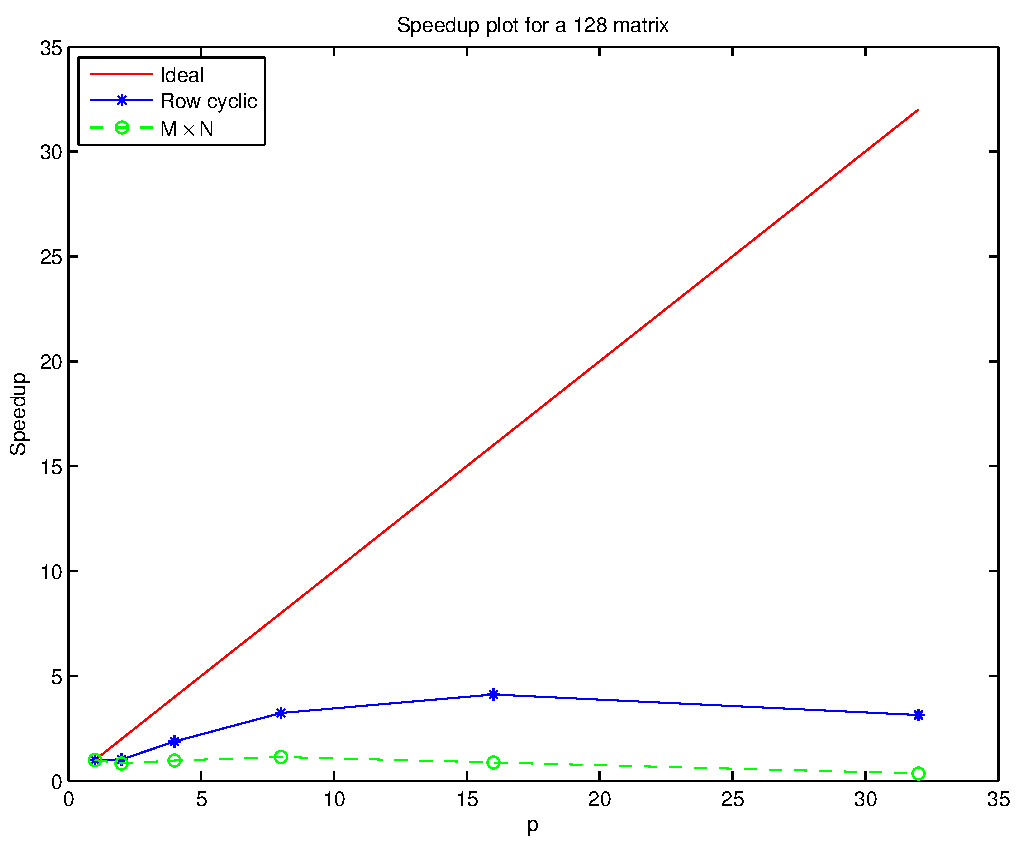
\includegraphics[scale=0.6]{img/128.pdf}
\caption{Speedup plot for a matrix $128\times128$.}
\end{center}
\end{figure}

\begin{figure}[H]
\begin{center}
 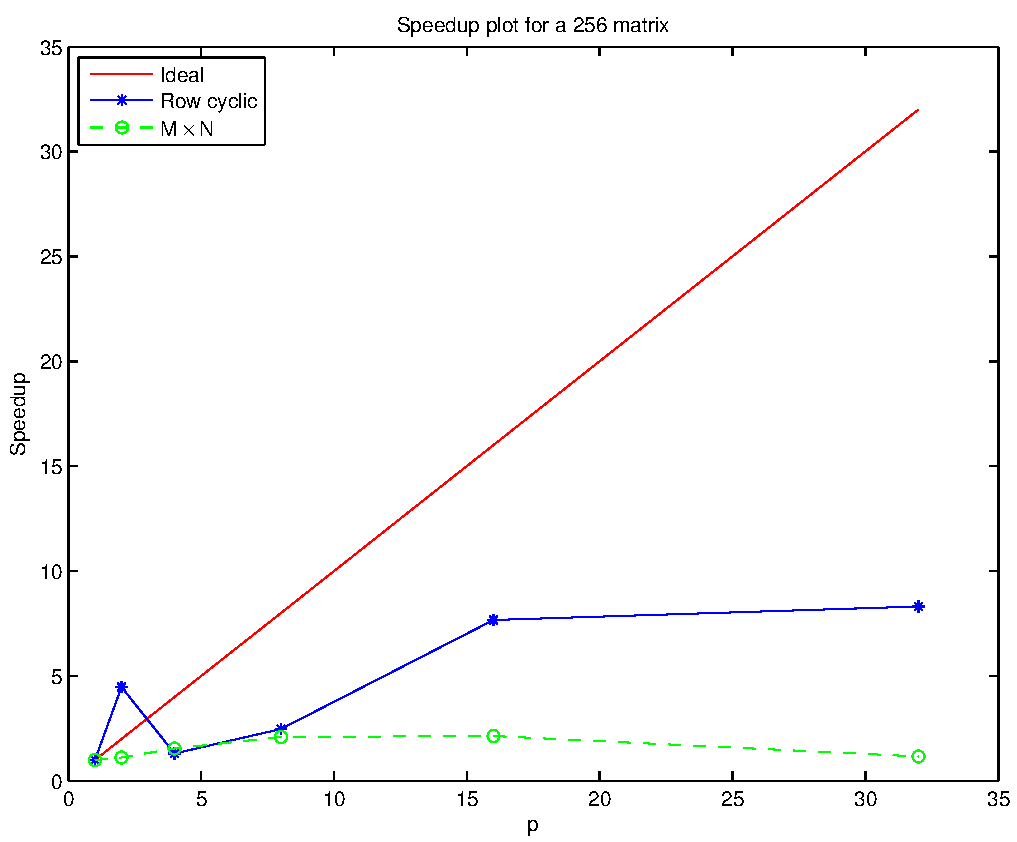
\includegraphics[scale=0.6]{img/256.pdf}
\caption{Speedup plot for a matrix $256\times256$.}
\end{center}
\end{figure}

\begin{figure}[H]
\begin{center}
 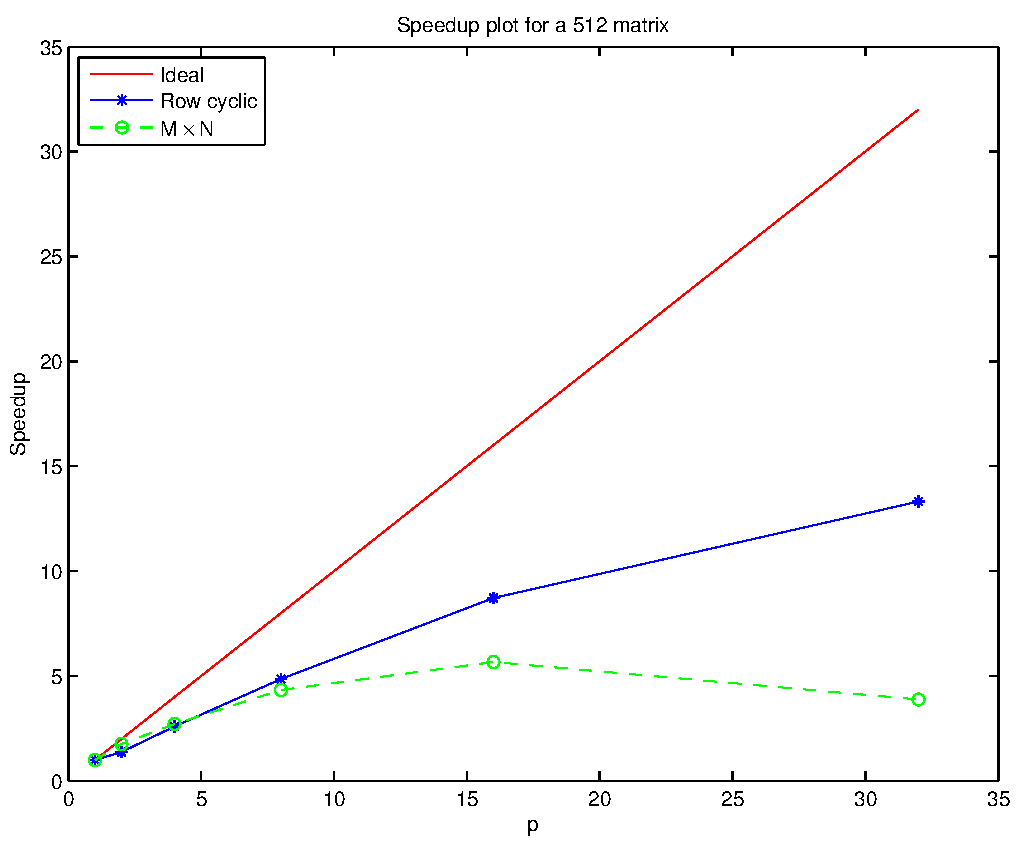
\includegraphics[scale=0.6]{img/512.pdf}
\caption{Speedup plot for a matrix $512\times512$.}
\end{center}
\end{figure}

\begin{figure}[H]
\begin{center}
 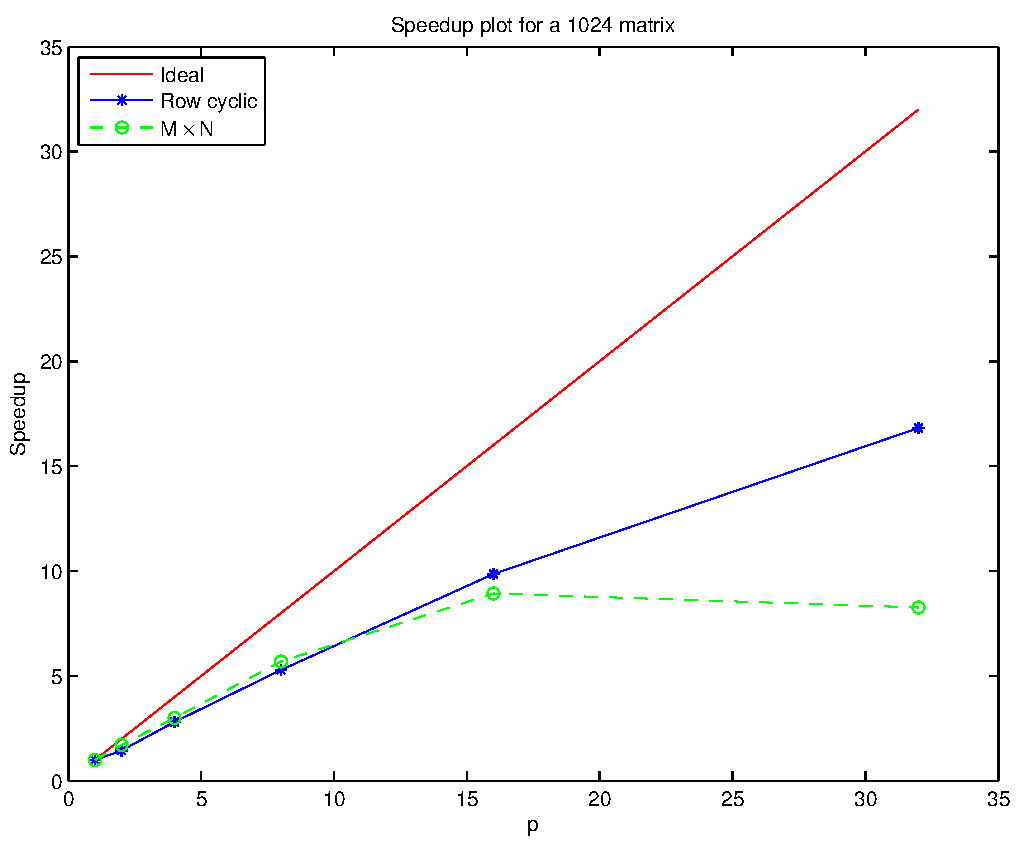
\includegraphics[scale=0.6]{img/1024.pdf}
\caption{Speedup plot for a matrix $1024 \times 1024$.}
\end{center}
\end{figure}

\begin{figure}[H]
\begin{center}
 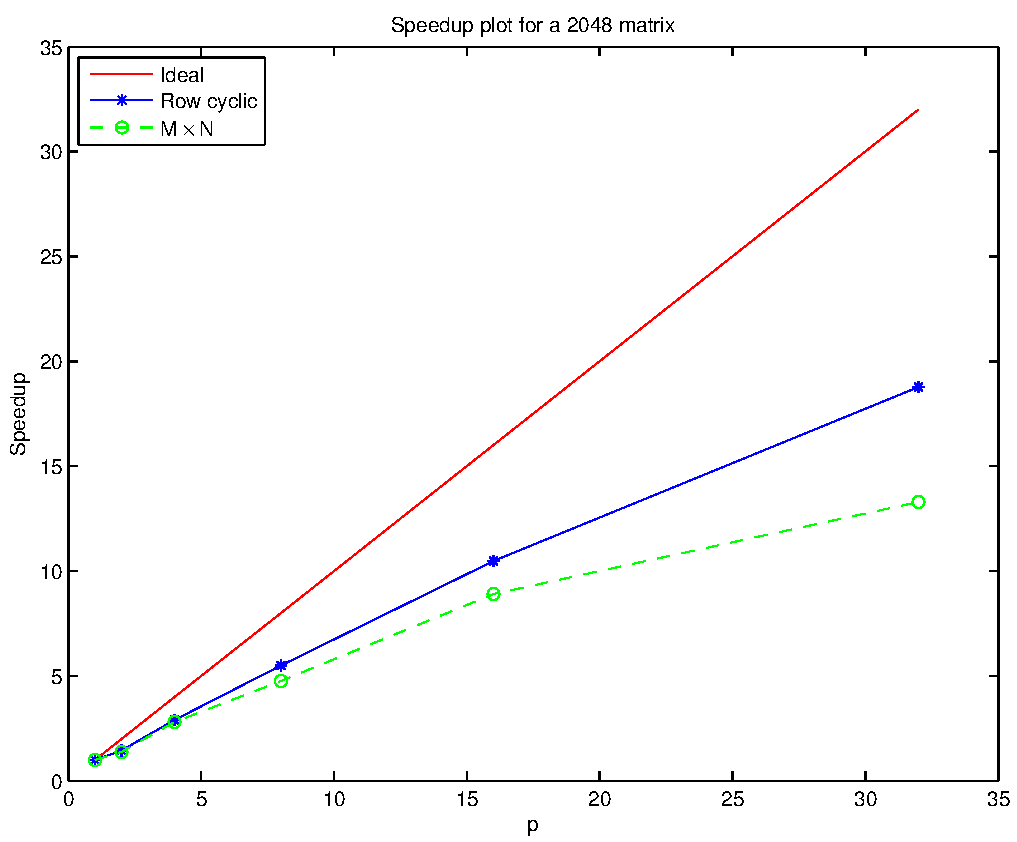
\includegraphics[scale=0.6]{img/2048.pdf}
\caption{Speedup plot for a matrix $2048 \times 2048$.}
\end{center}
\end{figure}

\begin{figure}[H]
\begin{center}
 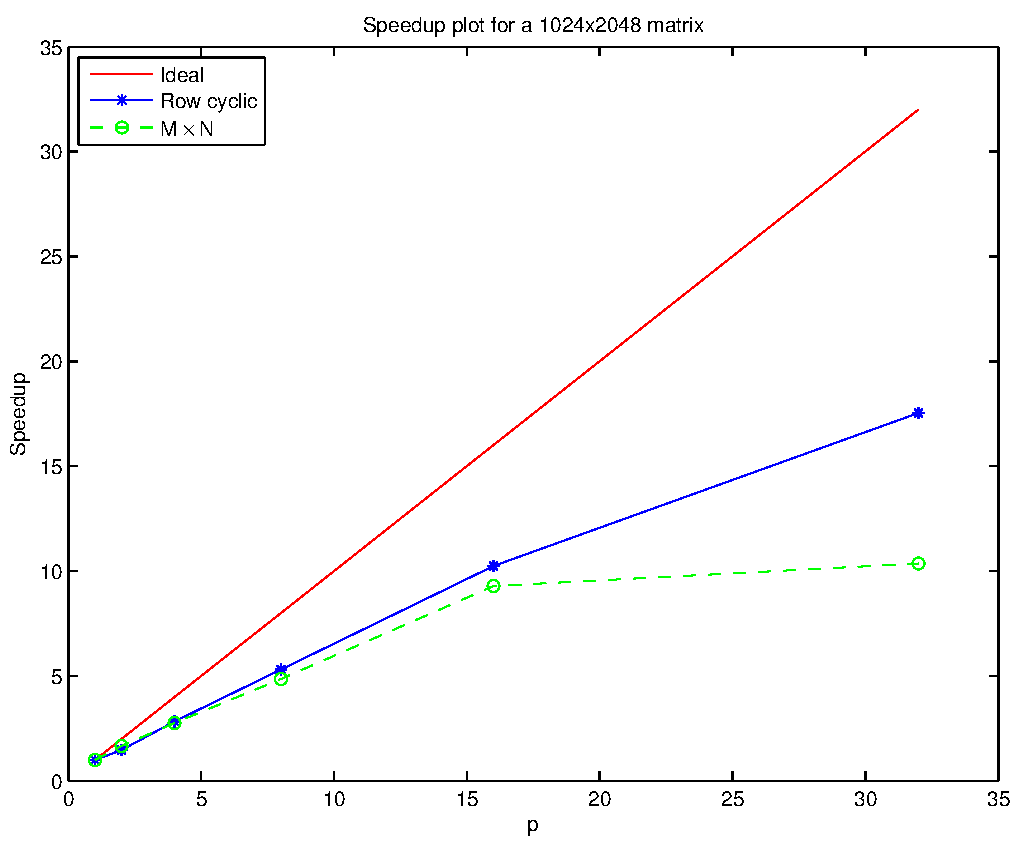
\includegraphics[scale=0.6]{img/1024x2048.pdf}
\caption{Speedup plot for a matrix $1024 \times 2048$.}
\end{center}
\end{figure}

\begin{figure}[H]
\begin{center}
 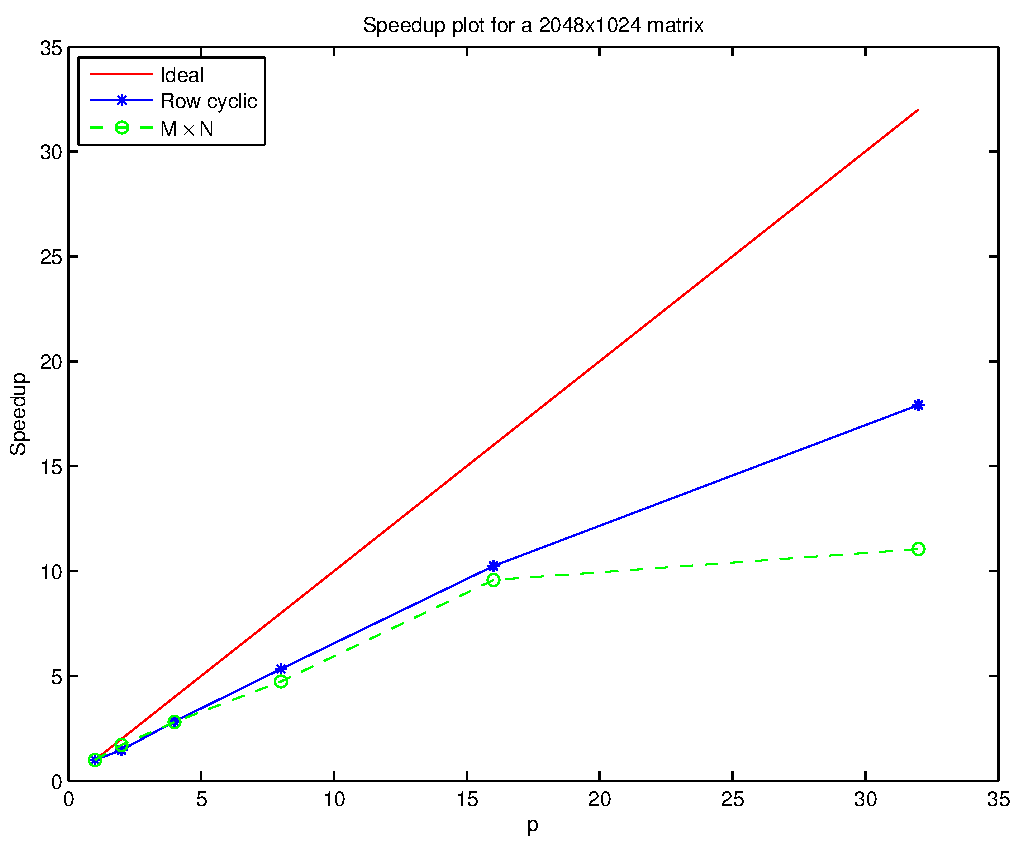
\includegraphics[scale=0.6]{img/2048x1024.pdf}
\caption{Speedup plot for a matrix $2048 \times 1024$.}
\end{center}
\end{figure}

\section{Conclusions and further developments}

From the numerical tests and the speedup plots it appears evident that a parallel approach toward the computation of the 2-Dimensional FFT is convenient: we have been able to speed up its computation considerably (for example, with the $2048 \times 2048$ matrix, in one case we improved from 2.2 to 0.1 seconds and in the other from $0.6$ to $0.05$ seconds).

We also have seen that, for relatively small sized problems ($128 \times 128$ and $256 \times 256$, for instance), probably it's better to avoid using too many processor, leaving them free for other programs to run, where their impact would be much greater.

In literature there exist many other implementation of the FFT that would probably lead to better performance: one of them is the famous ``Fast Fourier Transform in the West'' \footnote{\url{http://www.fftw.org/}} which provides both an implementation for  1D and 2D FFT. In that library there is already a parallel version of these implementations, aimed at SMP machines (like the one we used) for Cilk (a superset of C invented by one of the FFTW's creators aimed at easy parallelization and automatic load balancing between processors on shared memory machines) and MPI. For this reason, a comparison in both the implementation and the performance of our version of the 2D FFT and the one in FFTW could lead to even more insights about the exploitability of the parallelization for this particular operation.

\printbibliography
\end{document} 